\documentclass[10pt,twocolumn,letterpaper]{article}
\usepackage[pagenumbers]{cvpr}
%% This file contains a number of tweaks that are typically applied to the main document.
%% They are not enabled by default, but can be enabled by uncommenting the relevant lines.


%%
%% Official support for 2-column teaser figure
%%
\usepackage{cuted} %< for strip environment

%%
%% For auto-referencing of figures (see fig/teaser.tex and \label{} therein) 
%%
\usepackage{currfile} %< for \currfilebase macro

%%
%% caption and (global) spacing overrides
%%
\usepackage{caption} %< for "\captionof" commands (teaser)
% \setlength{\abovecaptionskip}{.5em} % space above caption
% \setlength{\belowcaptionskip}{1em} % space below caption

%%
%% Inline annotations; for predefined colors, refer to "dvipsnames" in the xcolor package:
%% https://tinyurl.com/overleaf-colors
%%
\newcommand{\red}[1]{{\color{red}#1}}
\newcommand{\todo}[1]{{\color{red}#1}}
\newcommand{\TODO}[1]{\textbf{\color{red}[TODO: #1]}}
%%
%% Disable for camera ready / submission by uncommenting these lines:
%%
% \renewcommand{\TODO}[1]{}
% \renewcommand{\todo}[1]{#1}

%%
%% Work harder in optimizing text layout. Typically shrinks text by 1/6 of page, enable
%% it at the very end of the writing process, when you are just above the page limit.
%%
% \usepackage{microtype}

%%
%% Fine-tune paragraph spacing.
%%
% \renewcommand{\paragraph}[1]{\vspace{.5em}\noindent\textbf{#1.}}

%%
%% Globally adjusts space between figure and caption.
%%
% \setlength{\abovecaptionskip}{.5em}

%%
%% Allows "the use of \paper to refer to the project name"
%% with automatic management of space at the end of the word.
%%
% \usepackage{xspace}
% \newcommand{\paper}{ProjectName\xspace}

%%
%% Commonly used math definitions.
%%
% \DeclareMathOperator*{\argmin}{arg\,min}
% \DeclareMathOperator*{\argmax}{arg\,max}

%%
%% Tighten underline.
%%
% \usepackage{soul}
% \setuldepth{foobar}

%%
%% Reconfigure paragraph (tweaks spacing)
%%
\usepackage{booktabs,graphicx,multirow,amsmath,array}
\usepackage{tikz}
\usetikzlibrary{positioning,arrows.meta}
\newcommand{\RawDevF}{0.625}
\newcommand{\NormDevF}{0.631}
\newcommand{\RawTestF}{0.6865}
\newcommand{\NormTestF}{0.6877}
\newcommand{\RawTestAcc}{0.681}
\newcommand{\NormTestAcc}{0.683}
\newcommand{\RawC}{0.25}
\newcommand{\NormC}{0.5}
\newcommand{\McNemarP}{0.82}
\newcommand{\FOnlyNorm}{90}
\newcommand{\FOnlyRaw}{86}
\newcommand{\PredChanged}{190}
\newcommand{\FDiffCI}{[-0.0073, +0.0096]}
\newcommand{\FDiff}{+0.0012}
\newcommand{\RulesTotal}{216}
\newcommand{\RulesObserved}{198}
\newcommand{\ChangedPct}{38.4}
\newcommand{\ChangedTest}{1127}
\newcommand{\ChangedAll}{7687}
\newcommand{\TokPerChanged}{1.6}
\newcommand{\NegLost}{0}
\newcommand{\NegRecovered}{8}
\newcommand{\ErrRaw}{956}
\newcommand{\ErrNorm}{952}
\newcommand{\Fixed}{90}
\newcommand{\Broken}{86}
\newcommand{\BrokenNeg}{35}
\newcommand{\CatSpell}{200}
\newcommand{\CatSlang}{146}
\newcommand{\CatNeg}{191}
\newcommand{\CatOther}{419}
\newcommand{\RobARaw}{92.1}
\newcommand{\RobANorm}{100.0}
\newcommand{\RobAN}{6393}
\newcommand{\WordRawF}{0.667}
\newcommand{\WordNormF}{0.672}
\newcommand{\WordRawAcc}{0.662}
\newcommand{\WordNormAcc}{0.667}
\newcommand{\ManualAudit}{94/100 preserved}
\newcommand{\GrpNeg}{10}
\newcommand{\GrpSpell}{129}
\newcommand{\GrpAbbr}{44}
\newcommand{\GrpSlang}{33}
\newcommand{\RobBARaw}{94.6}
\newcommand{\RobBANorm}{93.7}
\newcommand{\RobBAGain}{-0.9}
\newcommand{\RobBACI}{[-1.6, -0.2]}
\newcommand{\RobBBRaw}{93.4}
\newcommand{\RobBBNorm}{92.9}
\newcommand{\RobBBGain}{-0.4}
\newcommand{\RobBBCI}{[-1.1, +0.2]}
\newcommand{\RobBCRaw}{91.2}
\newcommand{\RobBCNorm}{91.1}
\newcommand{\RobBCGain}{-0.1}
\newcommand{\RobBCCI}{[-0.7, +0.6]}
\newcommand{\RobBDRaw}{87.9}
\newcommand{\RobBDNorm}{87.6}
\newcommand{\RobBDGain}{-0.4}
\newcommand{\RobBDCI}{[-1.0, +0.3]}
\newcommand{\RobAGain}{+7.9}
\newcommand{\RobACI}{[+7.2, +8.5]}
\newcommand{\RobAFRaw}{0.680}
\newcommand{\RobAFNorm}{0.688}
\newcommand{\RobAFOrigRaw}{0.687}
\newcommand{\RobAFOrigNorm}{0.688}
\newcommand{\ErrSpellWith}{30.7}
\newcommand{\ErrSpellWithout}{32.2}
\newcommand{\ErrSlangWith}{30.7}
\newcommand{\ErrSlangWithout}{32.2}
\newcommand{\ErrNegWith}{35.8}
\newcommand{\ErrNegWithout}{30.0}
\newcommand{\NegTestN}{976}
\newcommand{\ShareTrueNeutral}{40}
\newcommand{\ShareNeutralPred}{53}
\newcommand{\SubChgRaw}{0.697}
\newcommand{\SubChgNorm}{0.692}
\newcommand{\SubUnchRaw}{0.677}
\newcommand{\SubUnchNorm}{0.681}
\newcommand{\DNeg}{+0.002}
\newcommand{\DNeu}{+0.003}
\newcommand{\DPos}{-0.002}
\newcommand{\AblMinF}{0.681}
\newcommand{\AblMaxF}{0.691}
\newcommand{\AblOnlyNegF}{0.687}
\newcommand{\AblWOnlyNegF}{0.665}
\newcommand{\AblOnlySpellF}{0.681}
\newcommand{\AblWOnlySpellF}{0.666}
\newcommand{\AblOnlyAbbrF}{0.684}
\newcommand{\AblWOnlyAbbrF}{0.664}
\newcommand{\AblOnlySlangF}{0.686}
\newcommand{\AblWOnlySlangF}{0.664}
\newcommand{\AblOnlyElongF}{0.688}
\newcommand{\AblWOnlyElongF}{0.663}
\newcommand{\ChgNegation}{1,108}
\newcommand{\ChgSpelling}{3,636}
\newcommand{\ChgAbbreviation}{2,924}
\newcommand{\ChgEnglishSlang}{1,132}
\newcommand{\ChgElongation}{816}
\newcommand{\VocabVarShare}{2.4}
\newcommand{\TypesRed}{1.2}
\newcommand{\TypesRedTwo}{1.7}
\newcommand{\OOVRaw}{13.4}
\newcommand{\OOVNorm}{13.3}
\newcommand{\TrainTypesRaw}{33,567}
\newcommand{\TrainTypesNorm}{33,152}
\newcommand{\FixedChg}{38}
\newcommand{\BrokenChg}{43}
\newcommand{\FlipsChg}{85}
\newcommand{\FlipChgPct}{7.5}
\newcommand{\FlipUnchPct}{5.6}
\newcommand{\UnchN}{1,873}
\newcommand{\NetChg}{$-$5}
\newcommand{\FlipsUnch}{105}
\newcommand{\ChurnRefPct}{4.3}
\newcommand{\NegChgN}{476}
\newcommand{\FlipsChgNeg}{50}
\newcommand{\FixedChgNeg}{20}
\newcommand{\BrokenChgNeg}{26}
\newcommand{\FlipNegShare}{59}
\newcommand{\NegChgShare}{42}
\newcommand{\LCTenDiff}{+0.008}
\newcommand{\LCTenRaw}{0.616}
\newcommand{\LCTenNorm}{0.624}
\newcommand{\LCTenPos}{3/3}
\newcommand{\LCQuarterDiff}{+0.001}
\newcommand{\LCQuarterRaw}{0.646}
\newcommand{\LCQuarterNorm}{0.647}
\newcommand{\LCQuarterPos}{2/3}
\newcommand{\LCHalfDiff}{+0.002}
\newcommand{\LCHalfRaw}{0.666}
\newcommand{\LCHalfNorm}{0.668}
\newcommand{\LCHalfPos}{3/3}
\newcommand{\LCFullDiff}{+0.002}
\newcommand{\LCFullRaw}{0.685}
\newcommand{\LCFullNorm}{0.688}
\newcommand{\LCFullPos}{1/1}
\newcommand{\RobANegN}{1,235}
\newcommand{\RobANegRaw}{90.8}
\newcommand{\RobAOthN}{5,158}
\newcommand{\RobAOthRaw}{92.5}

\definecolor{cvprblue}{rgb}{0.21,0.49,0.74}
\usepackage[breaklinks,colorlinks,allcolors=cvprblue]{hyperref}
\def\confName{CVPR}
\def\confYear{2027}
\newcommand{\RepoURL}{https://github.com/Saumya0007/ML-PROJECT}

\title{Does Spelling Normalization Help Hinglish Sentiment Analysis?\\
Performance, Prediction Consistency and Meaning Preservation on SentiMix}

\author{Saumyadip Deb\\
IIT Jodhpur\\
{\tt\small m26cps007@iitj.ac.in}
\and
Ankit Kumar\\
IIT Jodhpur\\
{\tt\small m26cps002@iitj.ac.in}
\and
Anand Kumar Sah\\
IIT Jodhpur\\
{\tt\small m26csa001@iitj.ac.in}
}

\begin{document}
\maketitle

\begin{abstract}
Hinglish (Hindi--English) is written in Roman script with highly variable spelling, so one word may appear as \emph{nahi}, \emph{nhi} or \emph{nahin}. We ask whether conservative, dictionary-based spelling normalization improves a sentiment classifier, and whether it does so without altering the intended sentiment. Using the official SentiMix / SemEval-2020 Task~9 Hinglish split (20{,}000 tweets) and an identical TF--IDF + logistic-regression pipeline, we compare raw and normalized text on four axes: Macro-F1/accuracy, prediction consistency under spelling variants, class-wise behaviour, and a sentiment-preservation audit. Normalization rewrites \ChangedPct\% of all sentences, yet test Macro-F1 moves only from \RawTestF{} to \NormTestF{} (difference \FDiff, 95\% CI \FDiffCI, McNemar $p{=}\McNemarP$): no significant effect. Consistency under \emph{in-dictionary} variants rises from \RobARaw\% to \RobANorm\%, but this is by construction; under out-of-dictionary synthetic noise normalization gives no gain. The reason is coverage: the rules touch only \VocabVarShare\% of tokens and shrink the vocabulary by \TypesRed\%; a small gain appears only with 10\% of the training data (\LCTenDiff{} F1). The audit finds no lost negation token, and spelling variation is not the dominant error source. All code, seeds and results are released at \url{\RepoURL}.
\end{abstract}

\section{Introduction}
\label{sec:intro}
Social-media text in India is heavily code-mixed: Hindi words in Roman script are interleaved with English, with no standard orthography. A single word has many spellings (\emph{acha, accha, achha}), words are shortened (\emph{bahut}$\to$\emph{bht}), and letters are elongated (\emph{nahiiii}). A sentiment classifier that relies on surface forms may therefore predict differently for two spellings of the same sentence even though the meaning is unchanged. Standard metrics (accuracy, Macro-F1) do not expose this: they score each sentence once and say nothing about equivalent variants.

A natural remedy is \emph{spelling normalization}: map variants to a canonical form before classification~\cite{han2011lexical,eisenstein2013bad}. But normalization has risks: it may fail on slang, and an over-eager rule can silently change negation (\emph{nahi}, \emph{mat}) or sentiment-bearing words. We therefore evaluate normalization as an \emph{intervention} with three research questions:
\begin{itemize}\setlength\itemsep{0pt}
\item \textbf{RQ1} Does normalization change classification performance (Macro-F1, accuracy, per-class F1)?
\item \textbf{RQ2} Does it make predictions more consistent across meaning-preserving spelling variants?
\item \textbf{RQ3} Does it preserve sentiment, in particular negation?
\end{itemize}
\textbf{Contributions.} (i) A controlled raw-vs-normalized comparison with identical splits, features, classifier and tuning protocol; (ii) a transparent 216-entry normalization dictionary organised in rule groups, with an ablation over groups and over feature types; (iii) a consistency evaluation on two sets of spelling variants (in-dictionary and out-of-dictionary); (iv) a rule-level and sentence-level meaning-preservation audit and an error analysis. Our main finding is negative but informative: with character n-gram features, dictionary normalization neither helps nor hurts measurably.
\begin{table}[t]\centering\footnotesize\setlength{\tabcolsep}{3pt}
\begin{tabular}{@{}lp{6.2cm}@{}}
\toprule
RQ & Finding (details in Sec.~5)\\
\midrule
RQ1 & No significant change: Macro-F1 \RawTestF{} $\to$ \NormTestF{} (McNemar $p{=}\McNemarP$); no class favoured; small gain only with 10\% of the training data.\\
RQ2 & Consistency \RobARaw\%$\to$\RobANorm\% on in-dictionary variants (by construction); no gain on out-of-dictionary noise.\\
RQ3 & \NegLost{} negation tokens lost; 0 rule violations; flips concentrate in negation sentences in both directions.\\
\bottomrule
\end{tabular}
\caption{Summary of answers to the research questions.}\label{tab:rq}
\end{table}

\section{Literature Review}
\label{sec:lit}
\textbf{Code-mixed sentiment.} Early Hindi--English work combined lexicons with text normalization~\cite{sharma2015text}; Joshi et al.~\cite{joshi2016subword} instead learned sub-word (character n-gram) compositions and left spelling untouched. SemEval-2020 Task~9 (SentiMix)~\cite{patwa2020semeval} standardised evaluation on Hinglish and Spanglish tweets, and GLUECoS~\cite{khanuja2020gluecos} benchmarks code-switched NLP more broadly; multilingual encoders such as XLM-R~\cite{conneau2020unsupervised} and MuRIL~\cite{khanuja2021muril} are now common. Code-mixing and non-standard spelling are known difficulties for language identification~\cite{barman2014code}. Roman-script Hindi has no standard orthography, and SentiMix additionally contains hashtags, mentions, emoji and English slang, so the vocabulary is long-tailed.\\
\textbf{Normalization.} Work ranges from non-standard-word handling~\cite{sproat2001normalization} and lexical normalization of tweets~\cite{han2011lexical,baldwin2015shared} to code-mixed settings: Singh et al.~\cite{singh2018automatic} cluster Hindi--English spelling variants with word embeddings and report gains on POS tagging and sentiment, and van der Goot et al.~\cite{vandergoot2021lexical} study normalization of code-switched data for POS tagging. Eisenstein~\cite{eisenstein2013bad} asks whether to normalize the text or adapt the model; sub-word models~\cite{bojanowski2017enriching} are the model-side answer. Dictionary approaches are transparent but cover only listed forms; learned normalizers generalise at the cost of opacity and meaning drift.\\
\textbf{Robustness evaluation.} Models can be brittle to character-level noise~\cite{belinkov2018synthetic}, and behavioural testing~\cite{ribeiro2020checklist} checks invariance to meaning-preserving perturbations. Our consistency metric follows this idea.
\begin{table}[t]\centering\footnotesize\setlength{\tabcolsep}{2.5pt}
\begin{tabular}{@{}>{\raggedright\arraybackslash}p{0.8cm}>{\raggedright\arraybackslash}p{2.0cm}>{\raggedright\arraybackslash}p{2.0cm}>{\raggedright\arraybackslash}p{2.35cm}@{}}
\toprule
Work & Normalization & Task & Evidence reported\\
\midrule
\cite{sharma2015text} & rules + lexicon & Hi--En polarity & accuracy\\
\cite{joshi2016subword} & none (sub-word LSTM) & Hi--En sentiment & accuracy, F1\\
\cite{singh2018automatic} & unsupervised clusters & POS, sentiment & before/after scores\\
\cite{vandergoot2021lexical} & learned normalizer & code-switched POS & POS accuracy\\
\textbf{Ours} & audited 216-rule dictionary & SentiMix Hinglish sentiment & Macro-F1, significance, consistency, audit, churn\\
\bottomrule
\end{tabular}
\caption{Closest prior work vs.\ this study.}\label{tab:lit}
\end{table}
\textbf{Our novelty over prior work.} Earlier studies mostly ask \emph{whether a downstream score moves}. We treat normalization as a controlled intervention and add four things (to the best of our knowledge not combined before for Hinglish sentiment): (i)~a strong, tuned baseline (word+char TF--IDF) and paired significance tests (McNemar, bootstrap), plus a \emph{retraining-churn} reference that separates the effect of rewriting from ordinary refit noise; (ii)~a \emph{consistency} metric on attested (in-dictionary) and synthetic (out-of-dictionary) variants, so invariance is reported next to Macro-F1; (iii)~a rule-level and sentence-level \emph{meaning-preservation audit} with documented exclusions (Table~\ref{tab:excl}); (iv)~a coverage and data-efficiency explanation of \emph{when} normalization helps. Our finding is deliberately negative but informative: gains seen with weaker features do not carry over once character n-grams are used.

\section{Dataset and Preprocessing}
\label{sec:data}
We use the Hinglish track of SentiMix / SemEval-2020 Task~9~\cite{patwa2020semeval} with the \emph{official} splits (Table~\ref{tab:data}): 14{,}000 train, 3{,}000 dev and 3{,}000 test tweets labelled negative, neutral or positive (neutral is the largest class, 37.5\%). Files are in CoNLL style (one token per line); we rebuild each sentence from its token lines and join the separately distributed test labels by \texttt{uid}. We verified that no \texttt{uid} occurs in two splits.
\begin{table}[t]\centering\footnotesize\setlength{\tabcolsep}{4pt}
\begin{tabular}{lrrrr}
\toprule
Split & Neg. & Neu. & Pos. & Total\\
\midrule
Train & 4,102 & 5,264 & 4,634 & 14,000\\
Dev & 890 & 1,128 & 982 & 3,000\\
Test & 900 & 1,100 & 1,000 & 3,000\\
\midrule
All & 5,892 & 7,492 & 6,616 & 20,000\\
\bottomrule
\end{tabular}

\caption{SentiMix Hinglish class distribution per split.}\label{tab:data}
\end{table}

\textbf{Cleaning (both conditions).} Text is lowercased; URLs (split into tokens in this corpus) and \texttt{@user} mentions are replaced by placeholders. Emoji and punctuation are kept. A few training lines are noisy (e.g.\ non-Hinglish text with language tags); we keep them. This cleaning is identical for the raw and normalized conditions, so only the spelling rules differ.

\textbf{Leakage control.} Spelling variants used for the robustness test (Sec.~\ref{sec:robust}) are generated only from test sentences and are never used for training or tuning; all variants of one source sentence therefore stay in the test split.

\section{Method}
\label{sec:method}
\begin{figure}[t]\centering
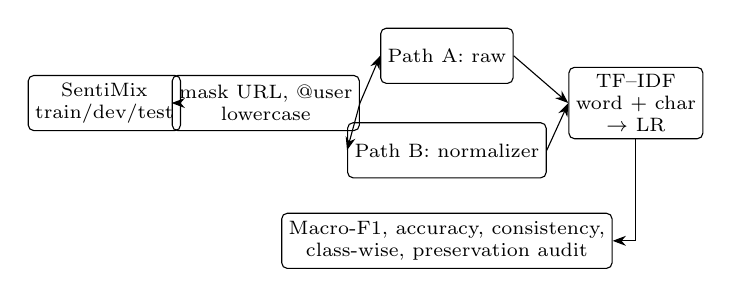
\begin{tikzpicture}[font=\scriptsize,>=Stealth,box/.style={draw,rounded corners=2pt,align=center,inner sep=2.5pt,minimum height=7mm}]
\node[box] (d) at (0,0) {SentiMix\\train/dev/test};
\node[box] (m) at (2.05,0) {mask URL, @user\\lowercase};
\node[box] (a) at (4.35,0.6) {Path A: raw};
\node[box] (b) at (4.35,-0.6) {Path B: normalizer};
\node[box] (c) at (6.75,0) {TF--IDF\\word + char\\$\to$ LR};
\node[box] (e) at (4.35,-1.75) {Macro-F1, accuracy, consistency,\\class-wise, preservation audit};
\draw[->] (d)--(m); \draw[->] (m.east)--(a.west); \draw[->] (m.east)--(b.west);
\draw[->] (a.east)--(c.west); \draw[->] (b.east)--(c.west); \draw[->] (c.south)|-(e.east);
\end{tikzpicture}
\caption{Controlled comparison: both paths share splits, masking, features, classifier and tuning; only the normalizer differs.}\label{fig:pipe}
\end{figure}

\textbf{Classifier.} Features are the union of word 1--2-gram TF--IDF~\cite{sparckjones1972statistical} (min\_df\,2, sublinear tf) and character 2--4-gram TF--IDF (\texttt{char\_wb}, min\_df\,3, $\le$150k features), fitted on train only. The classifier is multinomial L2-regularised logistic regression (scikit-learn~\cite{pedregosa2011scikit}, L-BFGS, \texttt{random\_state}=42). The inverse regularisation strength $C\in\{0.1,0.25,0.5,1,2\}$ is selected by dev Macro-F1 \emph{separately for each condition}; the model is then refit with that $C$ and evaluated once on test.

\textbf{Normalizer.} A token-level lookup maps spelling variants to one canonical form. Rules are organised in groups: \emph{negation} (\GrpNeg{} variants, e.g.\ \emph{nhi, nahin}$\to$\emph{nahi}), \emph{spelling} (\GrpSpell, e.g.\ \emph{acha, achha, accha}), \emph{abbreviation} (\GrpAbbr, vowel-dropped forms such as \emph{bht, kr, rha}), \emph{English slang} (\GrpSlang, e.g.\ \emph{plz, u, gud}) and \emph{elongation} (runs of $\ge3$ identical letters collapsed to two). Variants were mined from the training split by consonant-skeleton grouping and then reviewed by hand. Design rules: (a) conservative---only forms that almost always denote the same word; (b) negation words map only to negation words (checked automatically); (c) ambiguous forms are \emph{excluded}: \emph{na, ni, nai} (negation vs.\ other senses), \emph{ache} (English \emph{ache} vs.\ Hindi \emph{achhe}), \emph{kia} (\emph{kiya} vs.\ \emph{kya}), \emph{bs, hm, tm, m, s}, etc. Context inspection removed two candidate rules: \emph{ky} is Urdu \emph{ke}, not \emph{kya}, and \emph{shi} occurs in \emph{jai shi ram}.

\textbf{Procedure.} For each condition: (1)~mask and lowercase every sentence; (2)~[Path B only] split into alphabetic tokens, collapse runs of $\ge3$ identical letters, and replace each token found in the lookup by its canonical form, leaving all other characters untouched; (3)~fit the vectorizers on the training split, tune $C$ on dev, refit, predict test; (4)~store predictions and a checkpoint. Because the rewrite is a pure token-level substitution, the number and order of tokens never change, which makes the audit in Sec.~\ref{sec:audit} a simple token comparison.

\textbf{Metrics.} \emph{Macro-F1} (primary) and accuracy. \emph{Consistency}: for a pipeline $f$, original sentence $x$ and its variants $\mathcal V(x)$,
\begin{equation}
\mathrm{Cons}=\frac{1}{\sum_x|\mathcal V(x)|}\sum_{x}\sum_{v\in\mathcal V(x)}\mathbb 1\!\left[f(v)=f(x)\right],
\end{equation}
where $f$ includes the normalizer for Path B. \emph{Preservation}: a rule-level and sentence-level audit (Sec.~\ref{sec:audit}). Paired differences are tested with McNemar's test~\cite{mcnemar1947note} and a paired bootstrap~\cite{efron1993bootstrap} (2{,}000 resamples, seed 42).

\section{Experiments}
\subsection{Main comparison (RQ1)}
\begin{table}[t]\centering\footnotesize\setlength{\tabcolsep}{4pt}
\begin{tabular}{lcccc}
\toprule
Condition & $C$ & Dev F1 & Test F1 & Test Acc\\
\midrule
Raw text & 0.25 & 0.625 & 0.6865 & 0.6813\\
Normalized & 0.5 & 0.631 & 0.6877 & 0.6827\\
\bottomrule
\end{tabular}

\caption{Raw vs.\ normalized text (word + char features). $C$ chosen on dev.}\label{tab:main}
\end{table}
Table~\ref{tab:main} shows that normalization changes test Macro-F1 by \FDiff{} (bootstrap 95\% CI \FDiffCI) even though it rewrites \ChangedTest{} of the 3{,}000 test sentences. Of the 3{,}000 test predictions, \PredChanged{} change: \FOnlyNorm{} sentences become correct and \FOnlyRaw{} become wrong (McNemar $p{=}\McNemarP$). Dev favours normalization slightly (\RawDevF{} vs.\ \NormDevF) and so does test (\RawTestF{} vs.\ \NormTestF), but both gaps are within sampling noise; we conclude there is \emph{no detectable effect}. Test scores exceed dev scores for both conditions, as is common for this dataset; $C$ was tuned on dev only.

\textbf{Setup and sensitivity.} Everything runs on CPU (about 45\,s for both conditions). Table~\ref{tab:cdev} shows dev Macro-F1 over $C$: both conditions are flat for $C\in[0.1,1]$ (spread $\le$0.006), so the different selected values (\RawC{} vs.\ \NormC) reflect small dev differences rather than a different operating regime. scikit-learn's default word tokenizer discards one-character tokens, so rules such as \emph{h}$\to$\emph{hai} and \emph{u}$\to$\emph{you} also \emph{add} word features that the raw word-level model cannot see (the char n-grams still do); this is part of the intervention.
\begin{table}[t]\centering\footnotesize\setlength{\tabcolsep}{4pt}
\begin{tabular}{lccccc}
\toprule
$C$ & 0.1 & 0.25 & 0.5 & 1 & 2\\
\midrule
Raw & 0.621 & 0.625 & 0.624 & 0.622 & 0.612\\
Normalized & 0.625 & 0.626 & 0.631 & 0.627 & 0.613\\
\bottomrule
\end{tabular}

\caption{Dev Macro-F1 for each inverse regularisation strength $C$.}\label{tab:cdev}
\end{table}

\subsection{Why so little effect? Coverage}
\begin{table}[t]\centering\footnotesize\setlength{\tabcolsep}{4pt}
\begin{tabular}{lrr}
\toprule
 & Raw & Normalized\\
\midrule
Train word types & 33,567 & 33,152\\
Types with df$\ge$2 & 12,452 & 12,237\\
Test OOV tokens (df$\ge$2 vocab) & 13.4\% & 13.3\%\\
Train tokens covered by rules & \multicolumn{2}{c}{2.4\%}\\
\bottomrule
\end{tabular}

\caption{Vocabulary effect of normalization (train split, test OOV).}\label{tab:vocab}
\end{table}
\begin{table}[t]\centering\footnotesize\setlength{\tabcolsep}{3pt}
\begin{tabular}{lrrl}
\toprule
Group & Rules & Sent. changed & Examples\\
\midrule
Negation & 10 & 1,108 & \emph{nhi, nahin, nehi}\\
Spelling & 129 & 3,636 & \emph{acha, bohot, kyu, jese}\\
Abbreviation & 44 & 2,924 & \emph{bht, kr, rha, gya}\\
English slang & 33 & 1,132 & \emph{u, ur, plz, gud}\\
Elongation & regex & 816 & \emph{nahiii, yayyyy}\\
\bottomrule
\end{tabular}

\caption{Rule groups: number of variant forms and number of sentences (all splits) changed by each group alone.}\label{tab:groups}
\end{table}
Table~\ref{tab:vocab} gives a mechanistic reason. Tokens covered by a rule are only \VocabVarShare\% of the training tokens. Normalization shrinks the training vocabulary by just \TypesRed\% (\TypesRedTwo\% for types with df$\ge$2) and lowers the test out-of-vocabulary rate from \OOVRaw\% to \OOVNorm\%. Most unseen test tokens are names, hashtags, rare words and unlisted spellings that a conservative dictionary cannot cover. Although \ChangedPct\% of sentences contain at least one rewritten token (Table~\ref{tab:groups}), a typical rewrite is small (about \TokPerChanged{} tokens), so the feature space changes little.

\subsection{Ablation (RQ1)}
\begin{table}[t]\centering\footnotesize\setlength{\tabcolsep}{4pt}
\begin{tabular}{lccc}
\toprule
Configuration & Dev F1 & Test F1 & Test Acc\\
\midrule
\multicolumn{4}{l}{\emph{Word + char n-grams}}\\
Raw (no rules) & 0.625 & 0.686 & 0.681\\
\quad only Negation & 0.627 & 0.687 & 0.682\\
\quad only Spelling & 0.629 & 0.681 & 0.676\\
\quad only Abbreviation & 0.626 & 0.684 & 0.679\\
\quad only English slang & 0.626 & 0.686 & 0.681\\
\quad only Elongation & 0.626 & 0.688 & 0.683\\
All groups & 0.631 & 0.688 & 0.683\\
\quad $-$ Negation & 0.628 & 0.687 & 0.682\\
\quad $-$ Spelling & 0.630 & 0.682 & 0.677\\
\quad $-$ Abbreviation & 0.630 & 0.691 & 0.685\\
\quad $-$ English slang & 0.629 & 0.684 & 0.679\\
\quad $-$ Elongation & 0.630 & 0.686 & 0.681\\
\midrule
\multicolumn{4}{l}{\emph{Word n-grams only}}\\
Raw (no rules) & 0.616 & 0.667 & 0.662\\
\quad only Negation & 0.615 & 0.665 & 0.660\\
\quad only Spelling & 0.616 & 0.666 & 0.661\\
\quad only Abbreviation & 0.618 & 0.664 & 0.659\\
\quad only English slang & 0.620 & 0.664 & 0.660\\
\quad only Elongation & 0.615 & 0.663 & 0.658\\
All groups & 0.621 & 0.672 & 0.667\\
\bottomrule
\end{tabular}

\caption{Ablation. ``only $g$'': a single rule group; ``$-g$'': all groups except $g$. $C$ tuned on dev per row.}\label{tab:abl}
\end{table}
Table~\ref{tab:abl} compares rule groups and feature types. With word+char features every configuration lies between \AblMinF{} and \AblMaxF{} test Macro-F1, within the bootstrap uncertainty of the main comparison ($\approx\pm0.009$), so we cannot attribute a benefit or harm to any single group. Removing character n-grams lowers all scores by about 0.02, and normalization changes the word-only model from \WordRawF{} to \WordNormF{} Macro-F1 (accuracy \WordRawAcc{}$\to$\WordNormAcc). This difference is slightly larger than with char n-grams but of similar size as the noise level; it is consistent with, but does not prove, the hypothesis that character n-grams already absorb much spelling variation.

\subsection{Other classifiers (RQ1)}
To check that the conclusion is not specific to logistic regression, we repeated the raw-vs-normalized comparison with three other classifiers on the same word+char features and the same protocol (hyper-parameter chosen on dev, test evaluated once; \texttt{src/othermodels.py}): LinearSVC, Complement Naive Bayes and SGD with modified-Huber loss. The Macro-F1 differences ($-$0.0002, $-$0.0003, $+$0.0049) are of the same size as the bootstrap noise of the main comparison and have no consistent sign, so normalization again gives no reliable gain (Table~\ref{tab:othermodels}). Logistic regression was fixed as the main model beforehand; these runs are a robustness check, not a model search.
\begin{table}[t]\centering\footnotesize
\begin{tabular}{@{}lccc@{}}
\toprule
Classifier & Raw & Norm. & $\Delta$\\
\midrule
Logistic Reg. (main) & .6865 & .6877 & $+$.0012\\
LinearSVC & .6920 & .6918 & $-$.0002\\
ComplementNB & .6258 & .6255 & $-$.0003\\
SGD (mod.\ Huber) & .6473 & .6522 & $+$.0049\\
\bottomrule
\end{tabular}
\caption{Test Macro-F1 of other classifiers, raw vs.\ normalized text.}\label{tab:othermodels}
\end{table}

\subsection{Data efficiency (RQ1)}
If normalization mainly pools sparse variants, it should help most when training data is scarce. We train on random subsets (3 seeds; $C{=}0.5$ for both conditions) and evaluate on the full test set (Table~\ref{tab:lc}). With 10\% of the training data (1{,}400 tweets) normalization gains \LCTenDiff{} Macro-F1 and is ahead in \LCTenPos{} seeds; at 25\%, 50\% and 100\% the gain shrinks to \LCQuarterDiff, \LCHalfDiff{} and \LCFullDiff, below the uncertainty of the full-data comparison. This supports the pooling explanation, but with three seeds the low-resource result is indicative rather than conclusive.
\begin{figure}[t]\centering
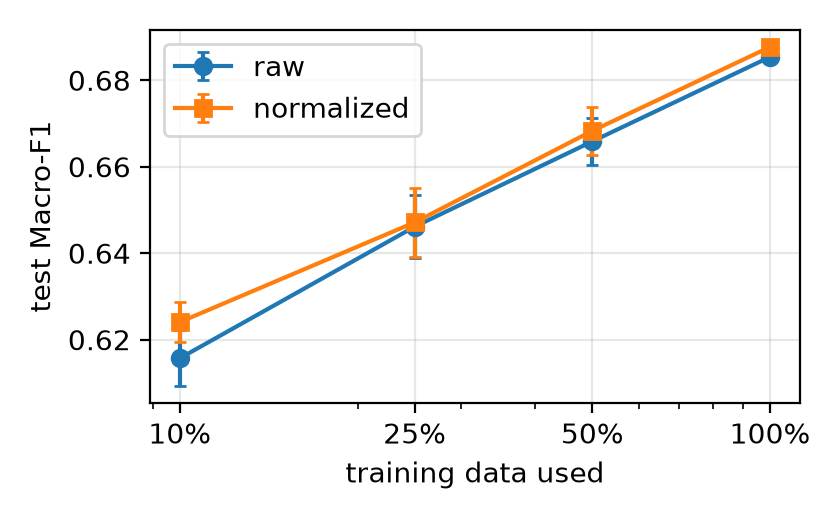
\includegraphics[width=0.8\linewidth]{../results/learning_curve.png}
\caption{Test Macro-F1 vs.\ amount of training data (mean$\pm$sd over 3 seeds).}\label{fig:lc}
\end{figure}
\begin{table}[t]\centering\footnotesize\setlength{\tabcolsep}{3pt}
\begin{tabular}{rrccc}
\toprule
Train frac. & $n$ & Raw F1 & Norm F1 & $\Delta$ (mean$\pm$sd)\\
\midrule
10\% & 1,400 & 0.616 & 0.624 & +0.008$\pm$0.003\\
25\% & 3,500 & 0.646 & 0.647 & +0.001$\pm$0.002\\
50\% & 7,000 & 0.666 & 0.668 & +0.002$\pm$0.001\\
100\% & 14,000 & 0.685 & 0.688 & +0.002\\
\bottomrule
\end{tabular}

\caption{Test Macro-F1 vs.\ training-set size (mean over seeds; $\Delta$=normalized$-$raw).}\label{tab:lc}
\end{table}

\subsection{Prediction consistency (RQ2)}
\label{sec:robust}
We build two variant sets from \emph{test} sentences. \textbf{Set A (attested swap)}: tokens belonging to a known spelling family are replaced by another family member (e.g.\ \emph{nahi}$\to$\emph{nhi}); up to three variants per sentence. Because the normalizer is built from the same families, A is an optimistic, in-dictionary upper bound. \textbf{Set B (synthetic noise)}: each word of length $\ge4$ is perturbed with probability $p$ by one of: drop an inner vowel, double a vowel, elongate the last letter, or a vowel-pair / \emph{v}$\leftrightarrow$\emph{w} / \emph{ph}$\leftrightarrow$\emph{f} substitution; three variants per sentence, $p\in\{0.1,0.2,0.3,0.5\}$. Most B variants are not in the dictionary. Variant generation is deterministic given the seed: for each test sentence and each of three draws, every eligible word is perturbed independently; draws that leave the sentence unchanged are discarded, which is why the number of variants is below three per sentence (Table~\ref{tab:rob}). A sample of 60 variants per set is stored for manual meaning checks (App.~\ref{app:var}). We evaluate the already-trained models (no retraining) and report consistency (Eq.~1) with a paired-bootstrap CI for the gain.
\begin{table}[t]\centering\footnotesize\setlength{\tabcolsep}{3pt}
\begin{tabular}{lrcccc}
\toprule
Variant set & $n$ & Raw & Norm. & Gain & 95\% CI\\
\midrule
A: attested swap & 6,393 & 92.1 & 100.0 & +7.9 & [+7.2, +8.5]\\
B: noise $p{=}0.1$ & 5,505 & 94.6 & 93.7 & -0.9 & [-1.6, -0.2]\\
B: noise $p{=}0.2$ & 7,603 & 93.4 & 92.9 & -0.4 & [-1.1, +0.2]\\
B: noise $p{=}0.3$ & 8,418 & 91.2 & 91.1 & -0.1 & [-0.7, +0.6]\\
B: noise $p{=}0.5$ & 8,869 & 87.9 & 87.6 & -0.4 & [-1.0, +0.3]\\
\bottomrule
\end{tabular}

\caption{Prediction consistency (\%) of raw vs.\ normalized pipelines under spelling variants. Gain in percentage points.}\label{tab:rob}
\end{table}
\begin{figure}[t]\centering
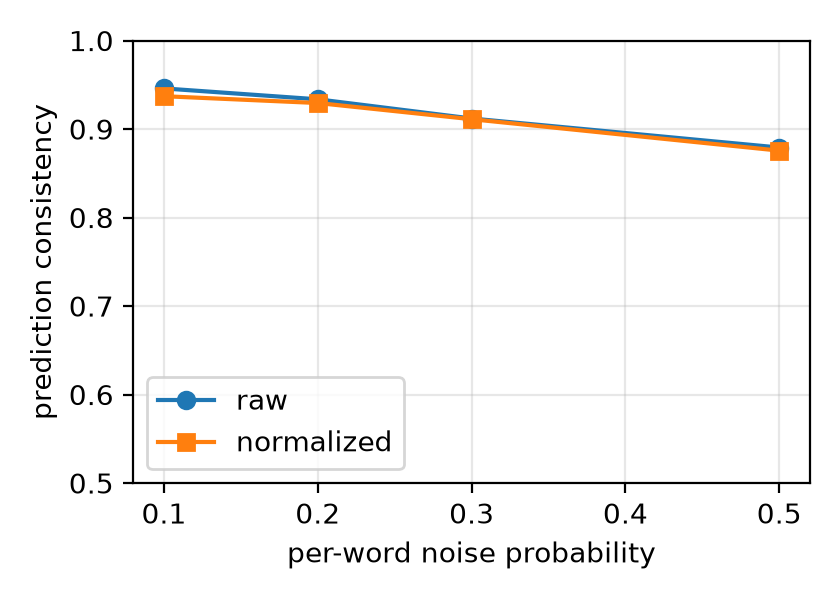
\includegraphics[width=0.78\linewidth]{../results/robustness_curve.png}
\caption{Consistency vs.\ noise level (Set B).}\label{fig:rob}
\end{figure}
Table~\ref{tab:rob} and Fig.~\ref{fig:rob} give two clear patterns. On Set~A, normalization raises consistency from \RobARaw\% to \RobANorm\% (gain \RobAGain{} points, CI \RobACI), and Macro-F1 on the variants from \RobAFRaw{} to \RobAFNorm; the 100\% is expected, since every Set-A variant maps back to the same normalized string. On Set~B, where noise is mostly outside the dictionary, there is no benefit: at $p{=}0.1$ the normalized pipeline is slightly \emph{less} consistent (\RobBAGain{} points, CI \RobBACI), and at $p\ge0.2$ differences are not distinguishable from zero. Breaking Set~A down by variant type, the raw model is less consistent when a \emph{negation} spelling changes (\RobANegRaw\% over \RobANegN{} variants) than for other families (\RobAOthRaw\% over \RobAOthN), the one place where spelling variation plausibly threatens sentiment; the normalizer removes this gap for listed variants. For Set~B, plausible explanations (not tested here) are: the raw model has learned in-vocabulary variant spellings as separate features, while normalization cannot recognise unseen noise; and character n-grams give both models similar tolerance. Both pipelines lose consistency steadily as noise grows (from about \RobBARaw\% to \RobBDRaw\% for raw).

\subsection{Class-wise analysis (RQ1)}
\begin{table}[t]\centering\footnotesize\setlength{\tabcolsep}{4pt}
\begin{tabular}{llccc}
\toprule
Class & Cond. & P & R & F1\\
\midrule
Negative & raw & 0.741 & 0.686 & 0.712\\
 & norm & 0.737 & 0.693 & 0.714\\
Neutral & raw & 0.587 & 0.651 & 0.618\\
 & norm & 0.591 & 0.654 & 0.621\\
Positive & raw & 0.750 & 0.711 & 0.730\\
 & norm & 0.752 & 0.705 & 0.728\\
\bottomrule
\end{tabular}

\caption{Per-class precision, recall and F1 on test.}\label{tab:cw}
\end{table}
Table~\ref{tab:cw} reports per-class results. Changes in F1 are tiny and of mixed sign (negative \DNeg, neutral \DNeu, positive \DPos), so normalization does not favour one sentiment class. Neutral is the hardest class under both conditions, and \ShareNeutralPred\% of raw errors are predictions of ``neutral''. Figure~\ref{fig:cw} visualises the F1 changes. Table~\ref{tab:conf} shows that the dominant confusions are between neutral and the polar classes under both conditions. This is class-wise analysis only, not a demographic fairness audit.
\begin{figure}[t]\centering
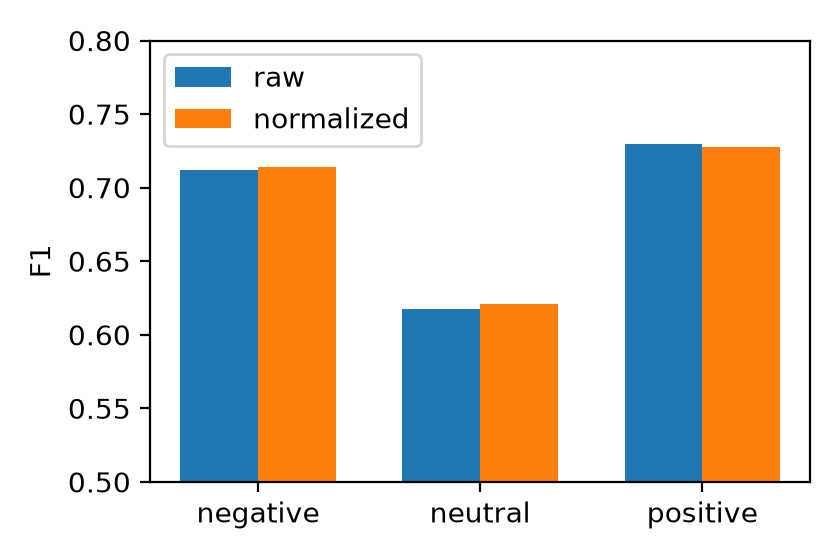
\includegraphics[width=0.78\linewidth]{../results/classwise_f1.png}
\caption{Class-wise test F1, raw vs.\ normalized.}\label{fig:cw}
\end{figure}
\begin{table}[t]\centering\footnotesize\setlength{\tabcolsep}{3pt}
\begin{tabular}{l|ccc|ccc}
\toprule
 & \multicolumn{3}{c|}{Raw (pred.)} & \multicolumn{3}{c}{Normalized (pred.)}\\
True & neg & neu & pos & neg & neu & pos\\
\midrule
neg & 617 & 245 & 38 & 624 & 236 & 40\\
neu & 185 & 716 & 199 & 189 & 719 & 192\\
pos & 31 & 258 & 711 & 34 & 261 & 705\\
\bottomrule
\end{tabular}

\caption{Confusion matrices on test (rows: gold).}\label{tab:conf}
\end{table}

\subsection{Sentiment-preservation audit (RQ3)}
\label{sec:audit}
\textbf{Rule level.} All \RulesTotal{} rules were checked automatically for negation compatibility (a negation token may only map to a negation token): 0 violations; \RulesObserved{} rules actually occur in the corpus. \textbf{Sentence level.} Normalization changes \ChangedAll{} of 20{,}000 sentences (\ChangedPct\%), on average \TokPerChanged{} tokens per changed sentence. The largest groups are spelling (\ChgSpelling{} sentences), abbreviation (\ChgAbbreviation) and English slang (\ChgEnglishSlang). The number of negation tokens is \emph{never lost} (\NegLost{} sentences) and increases in \NegRecovered{} sentences where an elongated negation (e.g.\ \emph{nahiii}) is recovered. These checks are partly guaranteed by construction; they verify the invariant, not semantic adequacy. \textbf{Manual sample.} We drew 100 changed test sentences (\texttt{results/audit\_sample.csv}) and one author labeled each as \emph{preserved}, \emph{not preserved} or \emph{unsure} (\texttt{results/audit\_sample\_labeled.csv}). \ManualAudit{} (94\%; 95\% Wilson CI [87.5\%, 97.2\%]), 4 were not preserved and 2 unsure. Of the sample, 42 sentences contain a negation token, and none of the six flagged cases changed a negation or the sentence polarity. The four \emph{not preserved} cases are word-level errors from ambiguous surface forms, not sentiment shifts: \emph{rha} in an English acronym was rewritten to \emph{raha}; \emph{sala} (``years old'') to \emph{saala} (an insult); and \emph{hn}, which here stands for \emph{hain} or \emph{hun}, to \emph{haan} (``yes'') in two sentences. The two \emph{unsure} cases involve \emph{u} and \emph{hun} that look like fragments of user handles. These show the main risk of context-free dictionary rules, namely homographs; the \emph{hn$\to$haan} rule is the most error-prone. The audit used a single labeler without inter-annotator agreement, so it is indicative only. The audit's main practical value was in rule design: reading rules in context removed \emph{ky} and \emph{shi} and motivated excluding \emph{ache}.

\subsection{Error analysis}\label{sec:err}
\begin{table}[t]\centering\footnotesize\setlength{\tabcolsep}{4pt}
\begin{tabular}{lrr}
\toprule
Primary category (raw errors) & Count & Share\\
\midrule
Other (context/sarcasm) & 419 & 43.8\%\\
Spelling variation & 200 & 20.9\%\\
Negation & 191 & 20.0\%\\
Slang/abbreviation & 146 & 15.3\%\\
\midrule
Total raw errors & 956 & 100\%\\
\bottomrule
\end{tabular}

\caption{Primary category of raw-model test errors (priority: spelling $>$ slang $>$ negation $>$ other).}\label{tab:err}
\end{table}
\begin{table}[t]\centering\footnotesize\setlength{\tabcolsep}{4pt}
\begin{tabular}{lrcc}
\toprule
Test subset & $n$ & Raw F1 & Norm F1\\
\midrule
Changed by rules & 1,127 & 0.697 & 0.692\\
Unchanged & 1,873 & 0.677 & 0.681\\
Contains negation & 976 & 0.588 & 0.592\\
Spelling variant & 652 & 0.697 & 0.696\\
Slang / abbrev. & 671 & 0.698 & 0.690\\
\bottomrule
\end{tabular}

\caption{Macro-F1 on test subsets (categories overlap).}\label{tab:sub}
\end{table}
We group the \ErrRaw{} raw-model errors (Table~\ref{tab:err}). The largest category, \CatOther{} errors, has no surface cue (context, sarcasm, neutral-vs-polar ambiguity); \CatSpell{} errors involve a spelling variant, \CatSlang{} slang/abbreviation or elongation, and \CatNeg{} negation. Spelling variation is not the dominant error source: the error rate is \ErrSpellWith\% for sentences with a variant token versus \ErrSpellWithout\% without (\ErrSlangWith\% vs.\ \ErrSlangWithout\% for slang). Negation sentences are harder (\ErrNegWith\% vs.\ \ErrNegWithout\%). \textbf{What does rewriting actually change?} The two models differ for two reasons: the rewritten text, and the fact that each is retrained (with its own $C$). We therefore separate the \ChangedTest{} rewritten test sentences from the \UnchN{} untouched ones. Among untouched sentences \FlipUnchPct\% of predictions (\FlipsUnch) still flip, which is pure retraining churn; refitting the raw pipeline with $C{=}0.5$ instead of the selected value flips \ChurnRefPct\% of all test predictions. Among rewritten sentences \FlipChgPct\% (\FlipsChg) flip: \FixedChg{} become correct and \BrokenChg{} become wrong (net \NetChg), so the excess flip rate attributable to rewriting is only about two points. Flips are over-represented in sentences with negation (\FlipNegShare\% of flips vs.\ \NegChgShare\% of rewritten sentences) but in both directions (\FixedChgNeg{} fixed vs.\ \BrokenChgNeg{} broken), which points to higher volatility of negation sentences rather than systematic harm from the rules; with such small counts we cannot exclude subtle effects. Table~\ref{tab:ex} shows examples. On the subset changed by rules, Macro-F1 is \SubChgRaw{} (raw) vs.\ \SubChgNorm{} (normalized); on unchanged sentences \SubUnchRaw{} vs.\ \SubUnchNorm{} (Table~\ref{tab:sub}).
\begin{table}[t]\centering\footnotesize\setlength{\tabcolsep}{3pt}
\begin{tabular}{@{}l p{2.9cm} p{1.6cm} c c c@{}}
\toprule
 & Tweet (excerpt) & Rules & Gold & Raw & Norm\\
\midrule
fixed & \scriptsize @u bikul sahi ji galtiya maf kiya ja skta hai par dokha kabhi bhi nhi so be happy and make & \scriptsize skta$\to$sakta, nhi$\to$nahi & neu & pos & neu\\
fixed & \scriptsize for all of ' emmaking stories of travelling in a car with music playing bhai sab gaane sun & \scriptsize h$\to$hai & neu & pos & neu\\
fixed & \scriptsize @u swamy ji k sath bahut galat hua bhale aadmio ki to koi ijjat hi nhi h . & \scriptsize nhi$\to$nahi, h$\to$hai & neg & pos & neg\\
broken & \scriptsize @u \# hny2 ki announcement hogyi to humka iss gola me nhi rehna hum nikal jaounga dusre go & \scriptsize nhi$\to$nahi & neu & neu & pos\\
broken & \scriptsize @u \_ fatiiiii nhi yaar yahan tw 1year walo k bhe khatam ho gye thy & \scriptsize fatiiiii$\to$fatii, nhi$\to$nahi, gye$\to$gaye & neu & neu & neg\\
broken & \scriptsize @u sunane main to yeh bhi aya hai bjp trolls are fired until 2023 kaphi kharcha ho gya nah & \scriptsize gya$\to$gaya & neu & neu & neg\\
\bottomrule
\end{tabular}

\caption{Test sentences whose prediction changed after rewriting (excerpts; offensive items omitted; @u = user mention).}\label{tab:ex}
\end{table}

\section{Discussion and Limitations}
Why does normalization not help? (1)~Coverage: the dictionary touches only \VocabVarShare\% of tokens and barely reduces OOV; (2)~character n-grams already generalise across close spellings; (3)~at corpus scale the common variants appear in training, so the model learns them directly (the pooling benefit shows only with 10\% of the data); (4)~most test errors are not spelling-related. Normalization is nevertheless useful as a \emph{guarantee}: in-dictionary variants receive identical predictions. \textbf{Limitations.} One dataset (tweets) and classical linear/NB classifiers only; no transformer baselines. The dictionary is hand-built for this corpus, so Set~A is optimistic and Set~B's meaning preservation is assumed from the perturbation types (a 60-sentence sample is provided for checking). Hyper-parameters were tuned per condition on dev only. Differences below $\approx$0.01 Macro-F1 are within bootstrap noise. The manual audit is small and, as a sample, cannot prove the absence of sentiment shifts. A stronger study would use human-written variants and larger code-mixed models.

\textbf{Threats to validity.} \emph{Internal:} the raw and normalized models are separate fits, so some prediction churn is unrelated to the rewrite (quantified in Sec.~\ref{sec:err}). \emph{Construct:} consistency measures invariance, not correctness; a pipeline that always predicts one class would be perfectly consistent. We therefore always report it next to Macro-F1 on the variants. \emph{External:} results may differ for other genres, other code-mixed pairs, or neural encoders with sub-word vocabularies. \textbf{Ethics.} The data are public tweets that contain abusive language. We mask user mentions, report no user identifiers, and omit offensive excerpts from the report.

\section{Conclusion}
A transparent 216-rule Hinglish spelling normalizer rewrites \ChangedPct\% of SentiMix sentences but does not significantly change TF--IDF + logistic-regression performance (Macro-F1 \RawTestF{} vs.\ \NormTestF{}), does not favour any class, preserves negation tokens by construction, and improves consistency only for in-dictionary variants. The rules cover just \VocabVarShare\% of tokens; the one setting where they help visibly is very low-resource training (10\% of the data, \LCTenDiff{} Macro-F1). Practitioners should therefore not expect accuracy gains from dictionary normalization when character n-grams are used, but may adopt it for deterministic handling of known variants.

\textbf{Practical guidance.} (i)~Do not rely on dictionary normalization for accuracy when character n-grams are available; (ii)~use it when deterministic handling of known variants or negation spellings matters, or when training data are very scarce; (iii)~always check candidate rules in context (two of our candidates were wrong) and keep ambiguous forms out; (iv)~report consistency next to Macro-F1, and compare against a retraining-churn reference before attributing prediction changes to the intervention.

\section*{Reproducibility Statement}
\textbf{Declaration.} All numbers, tables and figures in this report are produced by the scripts in the accompanying repository; no number was edited by hand. Experiments are CPU-only, deterministic (fixed seed 42, official splits, L-BFGS solver; \texttt{PYTHONHASHSEED}=0), and run in about 15 minutes on a laptop. Library versions are pinned in \texttt{requirements-lock.txt} (Python 3.12, scikit-learn 1.9.1, pandas 3.0.6, numpy 2.5.4). Datasets are \emph{not} included; they are public at Zenodo (record 3974927) and instructions are in \texttt{data/README.md}. Trained models (about 2\,MB each) are in \texttt{checkpoints/}. \textbf{To reproduce:} \texttt{pip install -r requirements.txt}; place the four data files in \texttt{data/}; run \texttt{python run\_all.py}; then compile \texttt{report/main.tex}. The repository is at \url{\RepoURL}. Commit hashes and timestamps are in Table~\ref{tab:commits}.

{\small\bibliographystyle{ieeenat_fullname}\bibliography{refs}}

\appendix
\section{Appendix}
\begin{table}[h]\centering\footnotesize\setlength{\tabcolsep}{4pt}
\begin{tabular}{@{}lll@{}}
\toprule
Hash & Timestamp & Message\\
\midrule
\texttt{d85f848} & 2026-11-08 15:58 & Add data loader and raw TF-IDF+LR baseline\\
\texttt{f11aa59} & 2026-11-08 17:08 & Add normalization rules, variant exploration, no\\
\texttt{1748f23} & 2026-11-09 12:58 & Add full experiment pipeline: ablation, robustne\\
\bottomrule
\end{tabular}

\caption{Repository commit history (hash, timestamp, message), generated by \texttt{src/commit\_log.py}.}\label{tab:commits}
\end{table}
\begin{table}[h]\centering\footnotesize\setlength{\tabcolsep}{4pt}
\begin{tabular}{lr}
\toprule
Quantity & Value\\
\midrule
Rules (variant forms) & 216\\
Rules observed in data & 198\\
Rules violating negation compatibility & 0\\
Sentences (all splits) & 20,000\\
Sentences changed & 7,687\\
\quad of which in test & 1,127\\
Changed by negation group & 1,108\\
Changed by spelling group & 3,636\\
Changed by abbreviation group & 2,924\\
Changed by English-slang group & 1,132\\
Changed by elongation & 816\\
Negation count unchanged & 7,679\\
Negation tokens lost & 0\\
Negation tokens recovered & 8\\
\bottomrule
\end{tabular}

\caption{Audit statistics (all numbers from \texttt{results/audit.json}).}\label{tab:audit}
\end{table}
\begin{table}[h]\centering\footnotesize\setlength{\tabcolsep}{4pt}
\begin{tabular}{@{}lp{5.6cm}@{}}
\toprule
Form & Why it is \emph{not} normalized\\
\midrule
\emph{na, ni, nai} & negation vs.\ tag particle / \emph{nayi} (``new'')\\
\emph{mat, mt} & imperative ``don't'' vs.\ other uses; kept as is\\
\emph{ache} & English \emph{ache} (pain) vs.\ \emph{achhe} (good)\\
\emph{kia} & \emph{kiya} vs.\ \emph{kya} vs.\ brand name\\
\emph{ky} & Urdu \emph{ke} (found in data), not \emph{kya}\\
\emph{shi} & \emph{jai shi ram} (found in data), not \emph{sahi}\\
\emph{bs, hm, tm} & \emph{bas}/BS, \emph{hum}/``hmm'', \emph{tum}/trademark\\
\emph{m, s, t} & fragments of English contractions (I'm, it's)\\
\emph{sale, km} & English \emph{sale} vs.\ \emph{saale}; \emph{km} = kilometres\\
\bottomrule
\end{tabular}
\caption{Ambiguous forms deliberately left unchanged (documented in \texttt{normalize.py}).}\label{tab:excl}
\end{table}
\begin{table}[h]\centering\footnotesize\setlength{\tabcolsep}{4pt}
\begin{tabular}{llr}
\toprule
Variant $\rightarrow$ canonical & Group & Freq.\\
\midrule
h $\rightarrow$ hai & abbreviation & 1,586\\
nhi $\rightarrow$ nahi & negation & 1,069\\
u $\rightarrow$ you & english\_slang & 832\\
wo $\rightarrow$ woh & spelling & 628\\
kr $\rightarrow$ kar & abbreviation & 545\\
kyu $\rightarrow$ kyun & spelling & 285\\
rha $\rightarrow$ raha & abbreviation & 218\\
apko $\rightarrow$ aapko & spelling & 213\\
ur $\rightarrow$ your & english\_slang & 160\\
sala $\rightarrow$ saala & spelling & 157\\
gya $\rightarrow$ gaya & abbreviation & 145\\
apke $\rightarrow$ aapke & spelling & 135\\
rhe $\rightarrow$ rahe & abbreviation & 128\\
plz $\rightarrow$ please & english\_slang & 127\\
\bottomrule
\end{tabular}

\caption{Most frequent normalization rules (frequency over all splits). Full list: \texttt{results/rule\_audit.csv}.}\label{tab:rules}
\end{table}
\begin{table}[h]\centering\footnotesize
\begin{tabular}{@{}l p{3.5cm} p{3.2cm}@{}}
\toprule
Set & Original (excerpt) & Token changes\\
\midrule
A & \scriptsize @u are koi ni @u apne yaha se terrorist to bhej hi sakte hi & \scriptsize sakte$\to$skte\\
A & \scriptsize thank you so much apka ek new india banane ke liye koti koti pradam apko & \scriptsize apko$\to$aapko\\
A & \scriptsize rt @u \_ singh \_ d @u 56 aate aate appostion wale bhag jate hai & \scriptsize wale$\to$waale, hai$\to$h\\
B & \scriptsize @u thank you priyanka ji feeling good .... & \scriptsize feeling$\to$feeleeng, good$\to$god\\
B & \scriptsize @u daang sorry to hear that . yea wish you best results ! & \scriptsize sorry$\to$sorryyy, best$\to$bst, results$\to$resoolts\\
B & \scriptsize @u imli ki chatniii but the best one is pudinay ki chatni dont fight me & \scriptsize best$\to$bst, dont$\to$doont\\
B & \scriptsize @u \_ predicament @u bade logo ki hoti hai tujh jese jhaatu newbie ko ghnta pata & \scriptsize hoti$\to$hti, jhaatu$\to$jhatu, rhega$\to$rheega\\
\bottomrule
\end{tabular}

\caption{Examples of generated variants (A: attested swap; B: synthetic noise, $p{=}0.3$).}\label{tab:variants}
\end{table}
\label{app:var}
\end{document}